\documentclass[runningheads]{llncs}
\usepackage[utf8]{inputenc}
\usepackage{graphics}
\usepackage{graphicx}
\usepackage{subcaption}
\usepackage{float}

\title{Tema 2-MyFileTransferProtocol (B)}
\author{Iordan Cosmina 2B1 }
\date{}
\institute{}

\begin{document}

\maketitle

\section{Introducere}

\par My file transfer protocol este o aplica\c{t}ie de tip client/server ce permite transferul de fi\c{s}iere \^{i}ntre clien\c{t}i \c{s}i server. 
\par Serverul acestei aplica\c{t}ii pune la dispozi\c{t}ie clien\c{t}ilor diferite comenzi cum ar fi \^{i}ntregistrarea,autentificarea \c{s}i diverse opera\c{t}ii cu directoare \c{s}i fi\c{s}iere( ex: deschiderea unui director, afi\c{s}area con\c{t}inutului unui director, transferul unui fi\c{s}ier). De asemenea acest server dispune de un mecanism de autorizare(ex: clien\c{t}ii care sunt \^{i}n "blacklist" nu se vor putea autentifica) \c{s}i un mecanism de ascundere a parolei la autentificare.
\par Un client nu v-a putea efectua nicio opera\c{t}ie dac\u{a} acesta este restric\c{t}ionat(se afla \^{i}n "blacklist"),dac\u{a} nu este \^{i}nregistrat sau dac\u{a} nu s-a autentificat. Dup\u{a} autentificare clientul se va putea folosii de toate opera\c{t}iile puse la dispozi\c{t}ie de server,iar la sfar\c{s}it acesta \^{i}\c{s}i va putea \^{i}ncheia sesiunea printr-o comand\u{a} de deconectare.
\par Aceast\u{a} aplica\c{t}ie este destinat\u{a} utilizatorilor ce vor s\u{a} transmit\u{a} fi\c{s}iere.

\section{Tehnologiile utilizate}

\par Pentru această aplicație voi folosi un protocol de tip TCP,deoarece este un protocol sigur orientat pe conexiune care permite ca un flux de octeți trimiși de pe o mașină să ajungă fără erori pe orice altă mașină din inter-rețea.
\par Modul de operare al protocolului TCP implică existența a trei faze. În prima fază, conexiunea trebuie stabilită , urmând un proces de confirmare pe baza mai multor pași. Imediat ce conexiunea a fost realizată, urmează transferul datelor. Odată ce transferul datelor s-a încheiat, conexiunea trebuie terminată în ideea de a închide calea virtuală și de a elibera resursele hardware/software implicate în proces.
\par O aplicație de tip FTP folosește 2 conexiuni TCP pentru a transfera date între server și clienți.
\begin{itemize}
  \item Conexiunea control,inițiată prin portul 21 ce permite trimiterea informațiilor de control (ex: parolă,username).
  \item Conexiunea de date,inițiată prin portul 20 ce permite transferul de date.
\end{itemize}
\par
\par Aspecte pozitive privind utilizarea TCP:
\begin{itemize}
  \item Este orientat conexiune.
  \item Oferă siguranță și asigură transmiterea în ordine a datelor.
  \item Oferă mecanisme de control al fluxului și control al congestiei.
  \item Este o arhitectură scalabilă, client-server. Acest lucru permite adăugarea rețelelor fără a perturba serviciile actuale.
 
\end{itemize}
\par Serverul TCP va crea câte un proces copil,folosind fork, pentru fiecare client pentru a putea servi mai mulți clienți simultan. Acesta va avea rolul de a prelua datele de la client,de a le procesa și,ulterior, de a trimite rezultatul către client.
\par Am ales acest protocol pentru ca este un serviciu de încredere care garantează livrarea unui flux de date trimis de la o gazdă la alta fără duplicarea sau pierderea de date.



\section{Arhitectura aplicatiei}

\par Pentru acest program se va instala o librărie ce are suport pentru protocolul FTP,diagramele de mai jos arată cum v-a funcționa codul,clientul va trimite comenzile către server,iar serverul va compila funcțiile în funcție de comenzile primite de la client,în diagrama server client este evidențiat acest aspect.

\begin{figure}[htp]
    \centering
    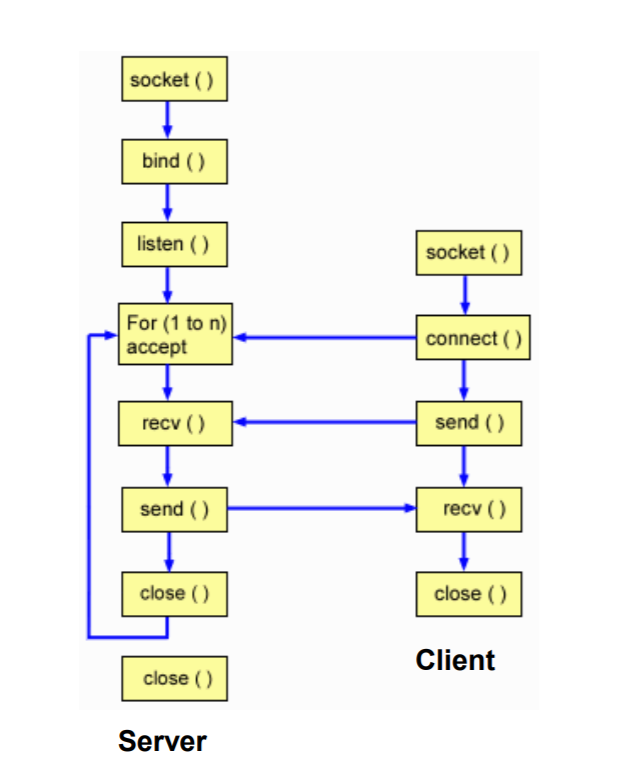
\includegraphics[width=6cm]{tcp.png}
    \caption{Modelul TCP client/server}
\end{figure}

\begin{figure}[htp]
    \centering
    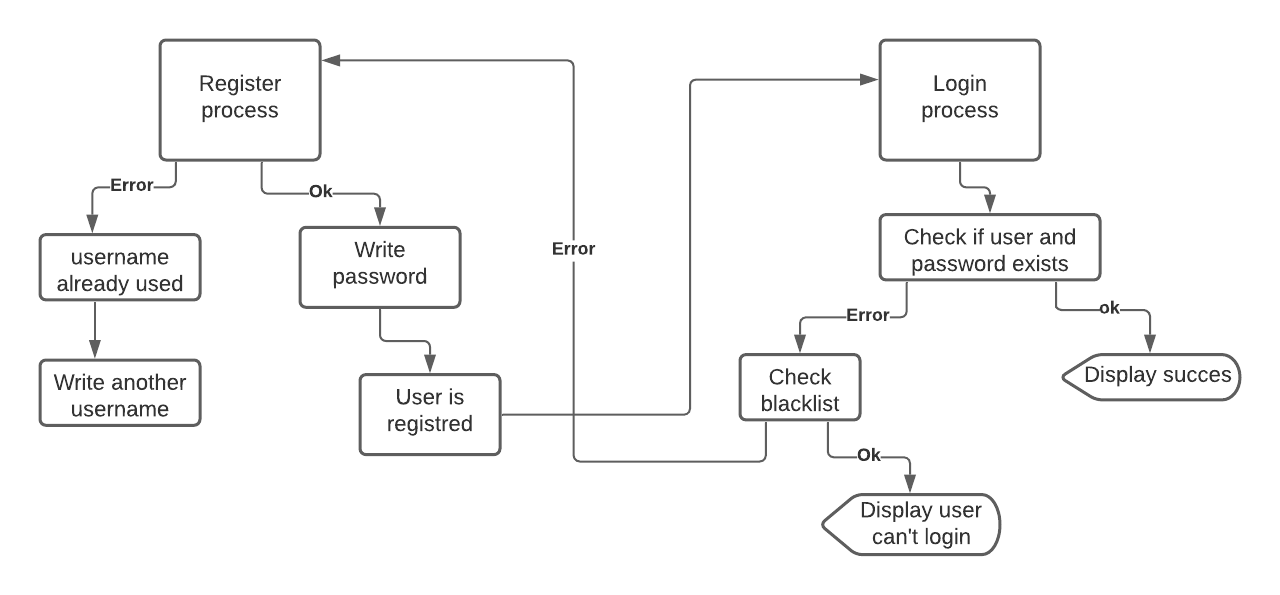
\includegraphics[width=13cm]{login.png}
    \caption{Diagrama login/register}
\end{figure}

\clearpage

\begin{figure}[H]
    \centering
    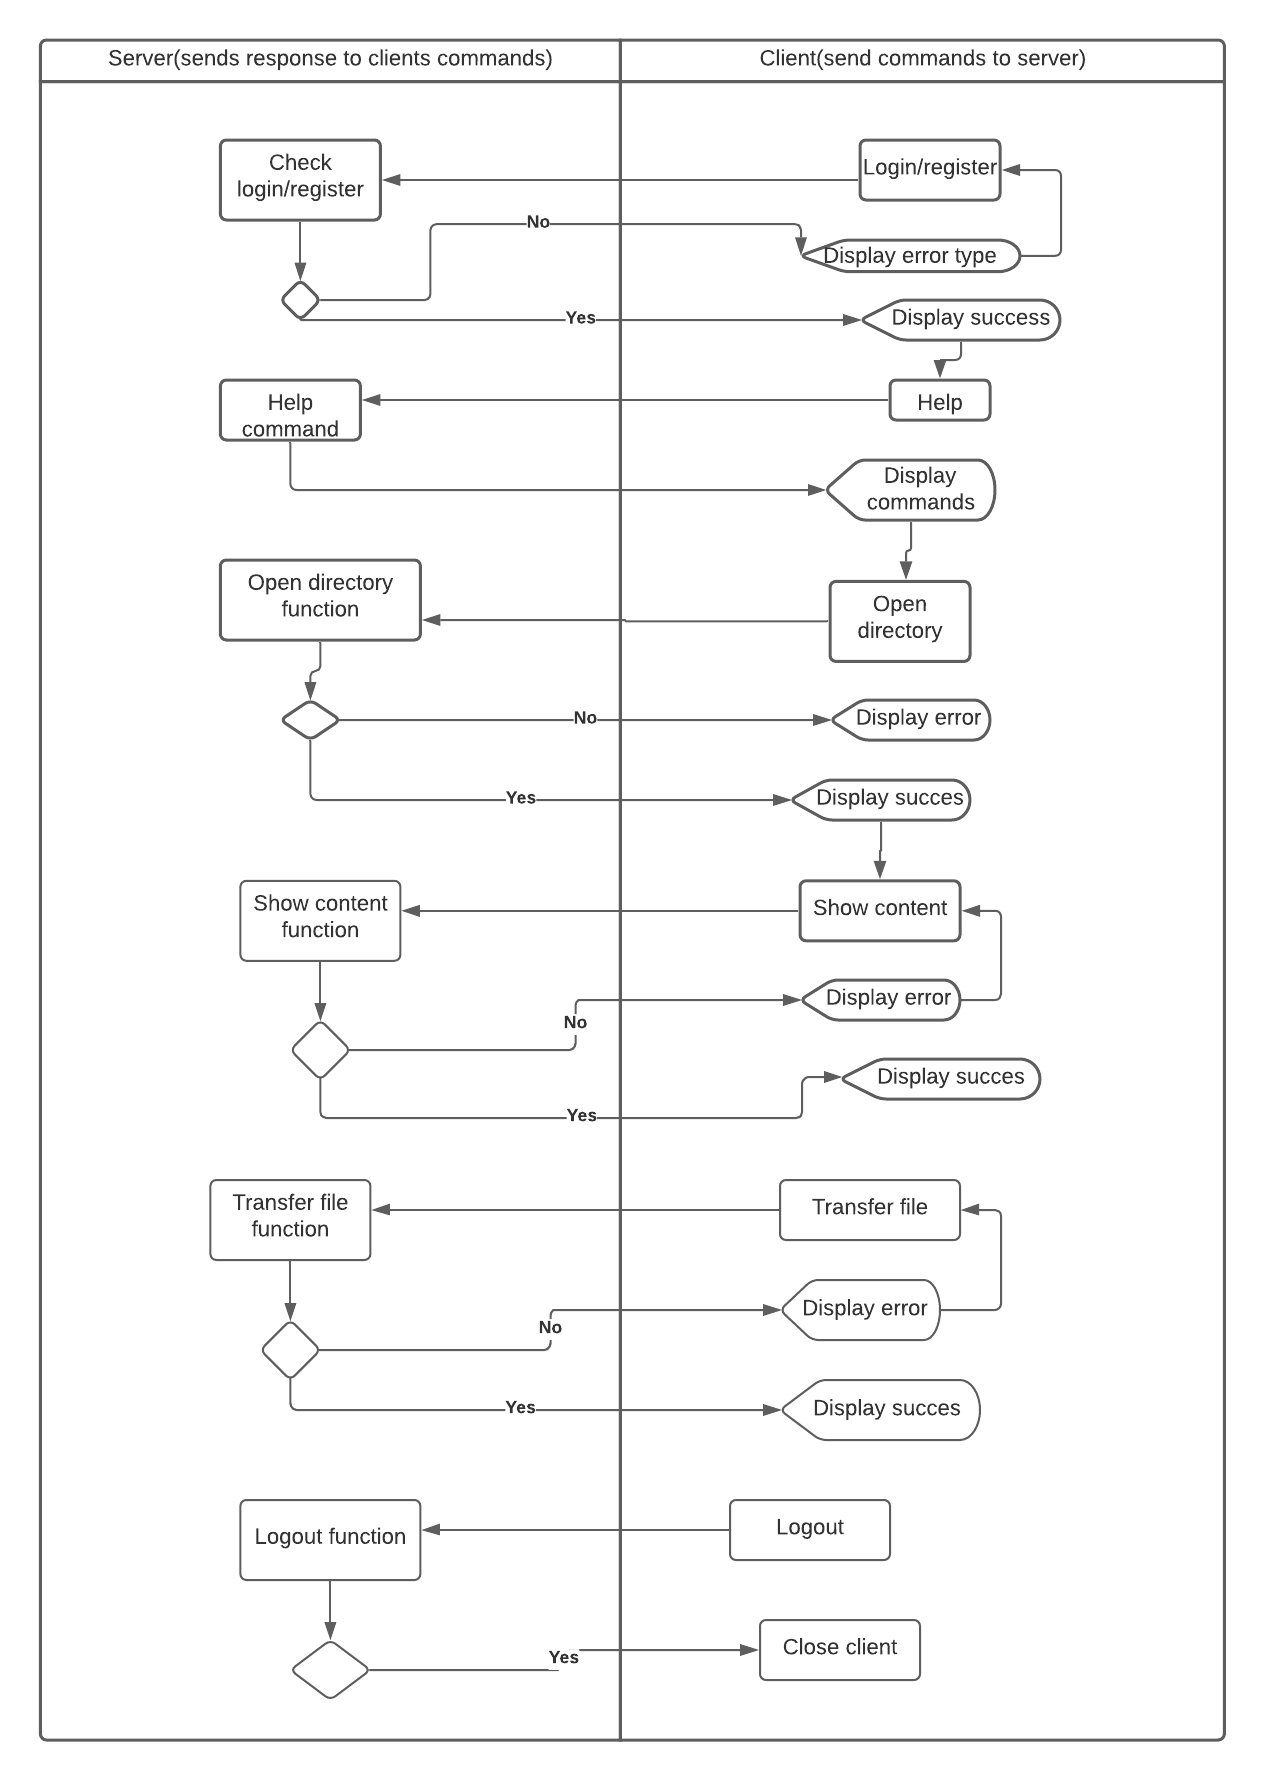
\includegraphics[width=13cm]{functions.png}
    \caption{Diagrama server/client}
\end{figure}


\newpage
\section{Detalii de implementare}
\par Pentru această aplicație voi folosi un protocol TCP concurent,astfel serverul va putea primi și executa comenzile mai multor clienți în același timp,rolul său fiind de a se fixa (bind) pe un port specific (port folosit de client pentru a localiza serverul) și de a asculta pentru noi conexiuni.
\par Acest server va primi de la client comenzi precum: register, login, help, logout, open directory, show directory content, transfer file.
\par Comanda \textit{\textbf{register}} va primi ca parametrii un username și o parolă(aceasta este "codată" în momentul scrierii,doar clientul va știi care este) și le va stoca într-un fișier cu conturile clienților,în același timp va verifica dacă există un alt client cu același username,dacă există clientul ce dorește înregistrarea va trebui să introducă un nou username până când se va găsi un username unic(nu mai există alt client cu acest username).
\par Comanda \textit{\textbf{login}} primește ca parametrii un user și o parolă pentru acestea verifică dacă există în fișierul cu conturi sau dacă sunt în fișierul cu conturi restricționate(blacklist). Dacă perechea \textit{username:parolă} se află în fișierul cu conturi atunci clientul este logat și folosi celelalte comenzi ale serverului,dacă această pereche se află în fișierul  cu conturi resticționate atunci clientul nu se va putea loga,conexiunea lui va fi întreruptă. De asemenea,la fel ca în cazul comenzii \textit{register} parola va fi "codată" astfel încât doar clientul va știi care este parola. Pentru implementarea acestei funcții voi folosi librăria \textit{conio.h}(este diferită față de librăria \textit{conio.h} disponibilă pentru Windows. Din această librărie mă folosesc de funcția \textit{getch()} pentru a obține codul ASCII al caracterului introdus de la tastatură fără că acesta să apară pe consola.
\par Comanda \textit{\textbf{help}} va afișa lista de comenzi disponibile pentru clienți.
\par Comanda \textit{\textbf{open directory}} va deschide directorul indicat de client prin numele acestuia sau prin calea acestuia. Dacă primește de la client numele directorului această comandă va căuta recursiv prin toate directoarele serverului și va returna succes când va găsi directorul. 
\par Comanda \textit{\textbf{show directory content}} va afișa pe ecranul clientului fișierele disponibile din directorul curent,sau în directorul a cărui cale acesta o trimite către server. Această funcție se comportă precum comanda "\textit{ls}" introdusă într-un terminal, listează toate directoarele și fișierele ce se află în directorul specificat.
\par Comanda \textit{\textbf{transfer file}} va permite serverului să trimită către client fișiere. Pentru transferul de date se folosește portul 20.Transferul se realizează utilizând modul de transfer activ (binar sau text).
\par Comanda \textit{\textbf{logout}} va deconecta clientul de la server și va închide procesul acestuia.

\par Un client nu va putea transmite către server comenzile pentru lucrul cu directoare dacă este restricționat sau dacă nu este autentificat. Deci comenzile \textit{\textbf{register}} și  \textit{\textbf{login}} sunt disponibile clienților imediat, iar restul comezilor vor fi disponibile îndată ce aceștia se conectează la server.

\section{Concluzii}
\par Această aplicație este destinată persoanelor ce doresc să transmită fișiere. Pentru îmbunătățire se mai pot adăuga diferite comenzi pentru operații cu directoare cum ar fi: ștergerea unui fișier/director, crearea unui fișier/director, afișarea mărimii unui director/fișier, redenumire, afișarea atributelor unui director/fișier, copierea conținutului unui fișier.

\section{Bibliografie}

Site-uri utilizate:
\begin{itemize}
  \item https: //profs.info.uaic.ro/~computernetworks/cursullaboratorul.php
  \item https://ro.wikipedia.org/wiki/Transmission\_Control\_Protocol
  \item https://github.com/zoelabbb/conio.h
  \item https://en.wikipedia.org/wiki/File\_Transfer\_Protocol\#Data\_transfer\_modes
  \item https://www.competentedigitale.ro/internet/internet\_ftp.php
  \item https://en.wikipedia.org/wiki/List\_of\_FTP\_commands
  \item https://tools.ietf.org/html/rfc959
  \item https://mbpfaus.net/~pfau/ftplib/
  
 
\end{itemize}

\end{document}
